\documentclass[11pt]{article}
\usepackage{fontspec}
\usepackage{xeCJK}
\setmainfont{Times New Roman}
\setCJKmainfont{Noto Serif SC}
\setCJKsansfont{Noto Sans SC}
\setCJKmonofont{Noto Sans SC}
\sloppy

\usepackage[a4paper,margin=1in]{geometry}
\usepackage{booktabs}
\usepackage{multirow}
\usepackage{amsmath}
\usepackage{amssymb}
\usepackage{graphicx}
\usepackage{tikz}
\usetikzlibrary{arrows.meta,positioning,fit,calc,shapes.geometric}
\usepackage{url}
\usepackage[hidelinks]{hyperref}

\title{面向版本化规范文档的本体语义漂移证据约束修复方法}
\author{匿名作者}
\date{}

\begin{document}
\maketitle

\begin{abstract}
版本化规范文档，例如技术标准、监管指南和协议规范，会持续修订定义、义务、例外、适用范围和生效条件。这类变化会使基于旧版本规范构建的 OWL 本体产生语义漂移：本体在语法上仍然有效，但其断言已经不再被当前规范证据支持。直接让大语言模型选择修复候选虽然实现简单，但难以审计，且容易受到候选描述、候选顺序、候选编号或隐含答案信息的影响。为解决这一问题，本文将本体语义漂移修复建模为一个证据约束的候选选择与形式化验证问题。

本文提出一种证据约束的语义中间表示本体修复方法。该方法首先基于公开规范证据进行谓词感知的证据聚焦，然后根据公开的 semantic type 与 predicate 将事件路由到时间版本、一般规则--例外、跨句作用域等任务表述；随后抽取原子事实，并转化为类型化语义中间表示；在语义结果固定后，系统才读取有限修复候选，并通过约束感知排序和选择性安全门控决定是否执行修复。被接受的修复还必须完成 OWL patch 物化、Reasoner 一致性检查、RDF 图差分验证和 competency question 回归验证。

在冻结 M16 方法后新构建的 RFC 真实规范文档 blind-large benchmark 上，ECR-Repair 在 264 个基于真实 RFC 规范文档构建并人工复核的修复事件、每个事件 5 次运行、共 1320 次调用中取得 1319/1320 的 OWL 修复闭环成功率，即 99.92\%，Wilson 95\% 置信区间为 99.57\%--99.99\%；严格事件成功率为 263/264，即 99.62\%，Wilson 95\% 置信区间为 97.89\%--99.93\%。消融实验显示，ECR-Repair 相对 M13 基础方法提升 22.50 个百分点，以事件为独立单位的配对 bootstrap 95\% 置信区间为 17.73--27.42 个百分点。候选 note 隔离审计、V4.3 离线排序 replay、补充的 DeepSeek/Ollama 后端替换、领域与来源族分组分析进一步表明，该方法不是依赖候选描述泄漏、固定编号或单一模型后端取得结果。
\end{abstract}

\section{引言}

本体常用于表示标准规范、监管规则、协议约束和领域知识。当其知识来源是规范文档时，本体的正确性不仅取决于逻辑一致性，还取决于其是否仍然被当前版本的规范证据支持。现实中，规范文档会不断更新：新版本可能替代旧版本，例外条款可能覆盖一般规则，限定语可能改变多个句子的作用域，或者某个属性值可能因为修订而失效。这些变化会导致本体出现语义漂移。

语义漂移不同于普通语法错误。本体可能仍然可以被 reasoner 正常加载，也没有明显的逻辑不一致，但其中某个属性值、规则约束或适用范围已经不再符合当前规范。对于这类问题，只做文本差异比较不够，只做 OWL consistency checking 也不够。系统需要理解规范文本中的版本关系、例外结构、作用域关系，并把这种理解转化为可验证的本体修复操作。

大语言模型为规范文本理解提供了新的可能，但直接使用 LLM 也带来风险。模型可能输出格式正确但语义失真的 JSON；可能因为候选描述写得更清楚而选择某个候选；可能受到候选顺序或编号的影响；也可能在证据不足时仍然给出确定修复。因此，本文不把问题简化为“让 LLM 直接选择答案”，而是将其拆解为证据理解、语义中间表示、候选映射、选择性门控和形式化验证等多个可审计阶段。

ECR-Repair 的核心思想是在候选修复进入模型决策之前，先固定候选盲的 evidence-grounded Semantic IR，并将候选选择限制在后续可审计、可弃权、可形式验证的决策层。这样，LLM 的作用被限定为证据解释和候选蕴含验证，而不是直接改写 OWL 本体或从候选集合中反向猜测答案。

本文研究问题可以表述为：

\begin{quote}
如何将版本化规范文档中的公开证据转化为可审计、候选隔离、可形式验证的 OWL 本体修复决策？
\end{quote}

本文主要贡献如下：

\begin{itemize}
    \item 提出面向版本化规范文档的本体语义漂移修复问题定义，将修复任务建模为证据约束的有限候选选择与 OWL 闭环验证问题。
    \item 设计证据约束的语义中间表示修复框架，包含谓词感知证据聚焦、任务表述路由、原子事实抽取、Semantic IR、约束感知候选排序、选择性安全门控、OWL patch、Reasoner 和 CQ 回归验证。
    \item 在方法冻结后构建并冻结一个更大规模 RFC 真实规范文档 blind-large benchmark，覆盖 264 个事件、11 个领域、13 个实际入选 RFC 来源族和三类语义漂移类型；构建阶段的候选来源注册表包含 69 条公开来源记录。
    \item 通过验证实验、消融实验、统计显著性检验、候选鲁棒性、模型后端对比、领域/来源族分组分析和失败分析，系统验证方法有效性与边界。
\end{itemize}

\section{相关工作}

\subsection{本体演化与本体修复}

本体演化研究关注知识库随领域变化而变化时如何保持一致性、可维护性和语义正确性\cite{flouris2008ontologychange,hartung2013ontologyevolution}。OWL 本体可以通过 reasoner 检查逻辑一致性\cite{w3cowl2}，但逻辑一致并不意味着语义仍然符合最新规范。已有本体修复研究多关注不一致公理删除、冲突定位、unsatisfiable concept repair 和 ontology alignment repair\cite{kalyanpur2006repair,jimenezruiz2015alignmentrepair}。SHACL 及其 repair 工作则从 RDF constraint validation 和 minimal repair 角度处理数据图约束违反\cite{w3cshacl2017,ahmetaj2022shaclrepair,ahmetaj2025shacllogic}。本文关注的问题不同：源本体未必不一致，但其断言相对于版本化规范文档已经过时。因此，本文同时要求候选选择正确、OWL 修改成功、reasoner 一致，并通过 competency question 回归验证修复闭环。

\subsection{RAG 与证据选择}

检索增强生成通常通过外部证据约束模型回答\cite{lewis2020rag}。近期研究指出，仅按相关性排序证据并不总是足够，因为最相关的片段未必最适合生成器进行推理。BAR-RAG 将 reranker 重新理解为边界感知证据选择器，强调选择对生成器“足够、可解、不过度泄漏”的证据\cite{sun2026barrag}。本文的谓词感知证据聚焦可以看作这一思想在规范文档本体修复任务中的领域化实现：系统不直接把全文交给模型，而是围绕 subject、predicate 和 case context 裁剪证据窗口。

\subsection{法律与监管信息抽取}

法律和监管文本中的信息抽取长期被认为具有挑战性，因为文本包含定义、义务、例外、条件、优先级和跨句作用域。Legal IE 相关综述指出，法律文本中的实体、关系和事件抽取仍然面临结构复杂、语言多样和跨句推理困难等问题\cite{premasiri2025legalie}。面向法律文本的 AMR 研究也表明，法律语义结构化需要处理领域词汇、角色关系和跨句语义\cite{vu2022legalamr}。De Jure 等监管规则抽取工作尝试将原始监管文本转化为结构化 rule set，并使用 LLM judge 和迭代修复提高质量\cite{guliani2026dejure}。法律需求翻译研究也使用 canonical representation 或 executable code 表示法律文本\cite{singhal2025legalrequirements}。本文与这些工作类似，都强调规范文本结构化；不同之处在于，本文的最终目标不是单独抽取规则，而是完成 OWL 修复候选选择和形式化闭环验证。

\subsection{大模型辅助本体工程}

大模型辅助本体工程研究关注如何使用 LLM 支持本体需求获取、概念生成、关系建模、本体评价和维护\cite{llmontology2026survey}。近期 ontology generation 工作进一步探索了从 user stories 和 competency questions 直接生成 OWL ontology draft 的可能性，并指出结构评价和专家评价仍然不可缺少\cite{lippolis2025ontologygeneration}。这类工作说明 LLM 能降低本体工程中的人工成本，但也暴露出 hallucination、结构不稳定和逻辑一致性不足等风险。本文采用更保守的定位：LLM 不直接修改本体，而是先生成可审计的 evidence-grounded Semantic IR；只有在候选隔离、形式化候选映射、选择性门控和 OWL closure 全部通过后，系统才接受修复。

\subsection{选择性预测与可信修复}

在高风险任务中，不确定时拒绝预测是一种合理机制。选择性预测研究关注模型在低置信度情况下 abstain，从而控制覆盖率与风险之间的权衡\cite{geifman2017selective}。本文将这一思想引入本体修复：只有当证据、Semantic IR、候选排序和 OWL 验证都满足约束时，系统才执行 patch；否则 fail-closed，避免错误修复污染本体。

\section{问题定义}

给定版本化规范文档集合 $D$、可能发生语义漂移的源本体 $O_0$，以及一个修复事件 $E$。每个事件包含公开元数据，包括 subject、predicate、semantic type、case context 和证据来源。对于每个事件，系统给定一个有限候选集合：

\[
C_E = \{c_1, c_2, \ldots, c_k\}.
\]

每个候选包含 display value 和形式化 OWL 编辑操作。私有 oracle 候选 $c_E^*$ 只在离线评价阶段读取，不能进入模型输入、候选排序之前的语义抽取阶段或人工提示。

方法输出可以是某个候选 $\hat{c}_E$，也可以是 abstain。若选择候选，则只有同时满足以下条件才记为修复闭环成功：

\begin{enumerate}
    \item 选择候选与私有 oracle 一致；
    \item 候选 OWL patch 成功物化；
    \item 修复后本体通过 reasoner 一致性检查；
    \item RDF 图差分反映了预期编辑；
    \item competency question 回归验证通过；
    \item 修复满足最小修改约束。
\end{enumerate}

本文报告三类指标：

\begin{itemize}
    \item 调用级 closure accuracy：每次运行是否完成完整修复闭环；
    \item oracle selection accuracy：每次运行是否选择 oracle candidate；
    \item strict event success：同一事件 5 次运行是否全部闭环成功。
\end{itemize}

\section{方法}

\subsection{总体框架}

本文将最终方法命名为 \textbf{ECR-Repair}（Evidence-Constrained Semantic IR Repair）。内部实验中，ECR-Repair 对应冻结的 \textbf{Full M16 configuration}，由四个层次组成；后文主结果表使用 ECR-Repair，M13/M14/M15/M16 仅作为消融阶段编号：

\[
\text{Evidence} \rightarrow \text{Semantic IR} \rightarrow \text{Candidate Decision} \rightarrow \text{OWL Closure}.
\]

\begin{figure}[t]
\centering
\resizebox{0.98\linewidth}{!}{%
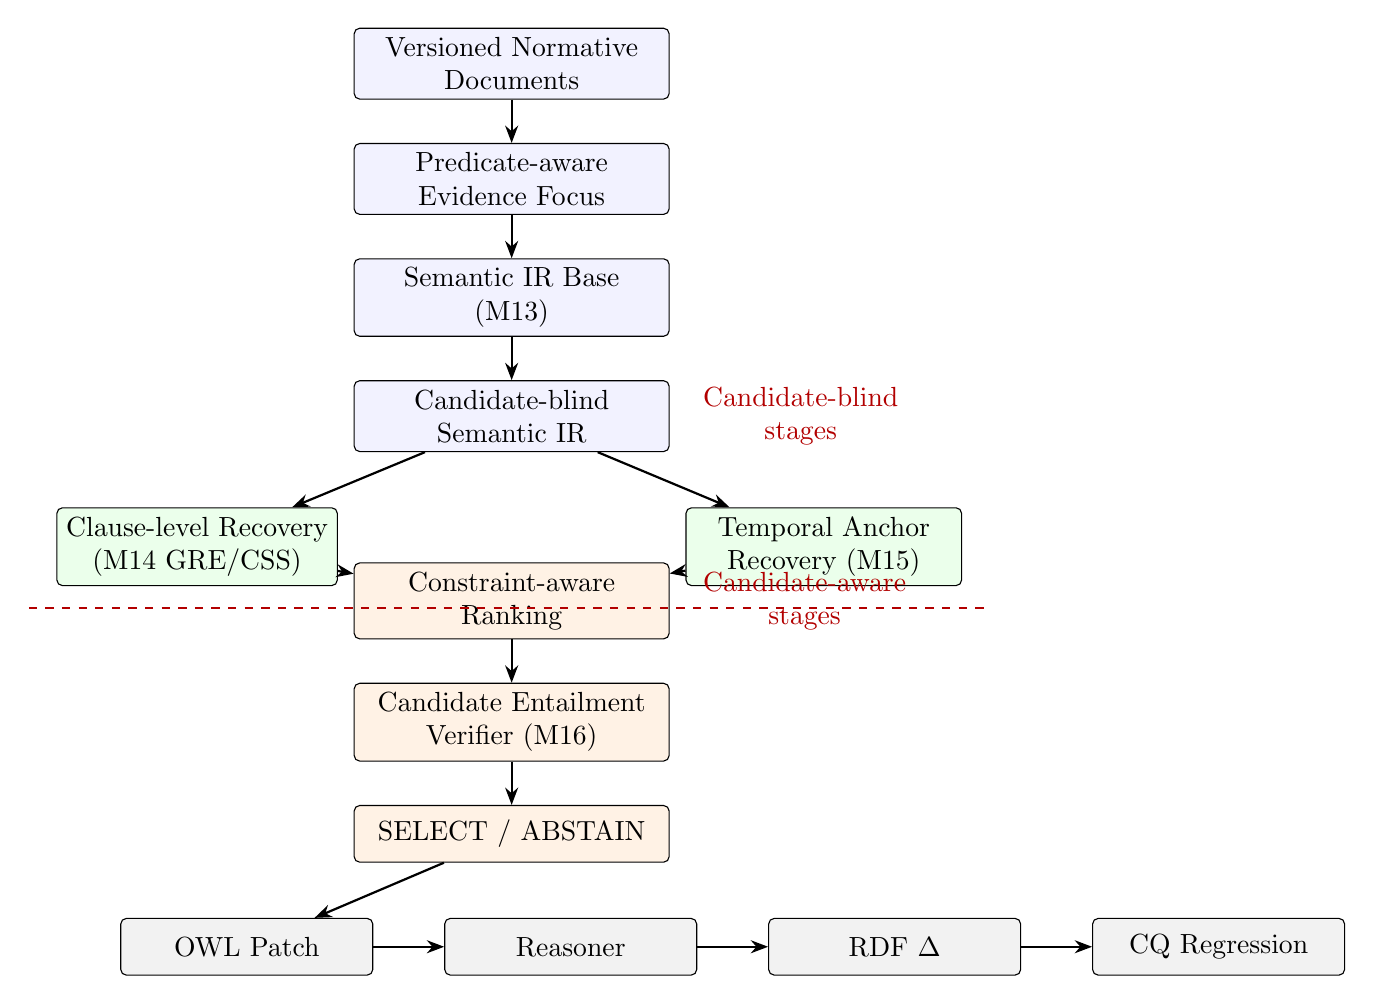
\begin{tikzpicture}[
    node distance=0.55cm and 0.9cm,
    box/.style={draw, rounded corners=2pt, align=center, minimum width=4.0cm, minimum height=0.72cm, fill=blue!5},
    branch/.style={draw, rounded corners=2pt, align=center, minimum width=3.5cm, minimum height=0.72cm, fill=green!8},
    aware/.style={draw, rounded corners=2pt, align=center, minimum width=4.0cm, minimum height=0.72cm, fill=orange!10},
    verify/.style={draw, rounded corners=2pt, align=center, minimum width=3.2cm, minimum height=0.72cm, fill=gray!10},
    arrow/.style={-{Stealth[length=2.2mm]}, thick},
    fence/.style={red!70!black, dashed, thick}
]
\node[box] (docs) {Versioned Normative\\Documents};
\node[box, below=of docs] (focus) {Predicate-aware\\Evidence Focus};
\node[box, below=of focus] (m13) {Semantic IR Base\\(M13)};
\node[box, below=of m13] (ir) {Candidate-blind\\Semantic IR};
\node[branch, below left=0.7cm and 0.2cm of ir] (m14) {Clause-level Recovery\\(M14 GRE/CSS)};
\node[branch, below right=0.7cm and 0.2cm of ir] (m15) {Temporal Anchor\\Recovery (M15)};
\node[aware, below=1.4cm of ir] (rank) {Constraint-aware\\Ranking};
\node[aware, below=of rank] (m16) {Candidate Entailment\\Verifier (M16)};
\node[aware, below=of m16] (decision) {SELECT / ABSTAIN};
\node[verify, below left=0.7cm and -0.25cm of decision] (patch) {OWL Patch};
\node[verify, right=of patch] (reasoner) {Reasoner};
\node[verify, right=of reasoner] (delta) {RDF $\Delta$};
\node[verify, right=of delta] (cq) {CQ Regression};

\draw[arrow] (docs) -- (focus);
\draw[arrow] (focus) -- (m13);
\draw[arrow] (m13) -- (ir);
\draw[arrow] (ir) -- (m14);
\draw[arrow] (ir) -- (m15);
\draw[arrow] (m14) -- (rank);
\draw[arrow] (m15) -- (rank);
\draw[arrow] (rank) -- (m16);
\draw[arrow] (m16) -- (decision);
\draw[arrow] (decision) -- (patch);
\draw[arrow] (patch) -- (reasoner);
\draw[arrow] (reasoner) -- (delta);
\draw[arrow] (delta) -- (cq);

\draw[fence] ($(m14.south west)+(-0.35,-0.28)$) -- ($(m15.south east)+(0.35,-0.28)$);
\node[red!70!black, align=center, right=0.3cm of rank] {Candidate-aware\\stages};
\node[red!70!black, align=center, right=0.3cm of ir] {Candidate-blind\\stages};
\end{tikzpicture}}
\caption{ECR-Repair 总体框架与候选隔离边界}
\label{fig:framework}
\end{figure}

具体流程如下：

\begin{center}
\begin{tabular}{ll}
\toprule
阶段 & 作用 \\
\midrule
谓词感知证据聚焦 & 根据 subject、predicate 和 case context 裁剪公开证据 \\
任务表述路由 & 将事件路由到时间版本、规则例外或作用域任务 \\
原子事实抽取 & 从聚焦证据中抽取 evidence-grounded facts \\
Semantic IR & 将事实转化为类型化中间语义表示 \\
约束感知排序 & 根据语义类型和本体约束给候选打分 \\
选择性门控 & 证据和候选不充分一致时拒绝修复 \\
OWL patch & 将候选操作物化为 OWL/RDF 修改 \\
Reasoner + CQ & 检查一致性和 competency question 回归 \\
\bottomrule
\end{tabular}
\end{center}

\begin{table}[t]
\centering
\caption{Evidence-constrained ontology repair 算法}
\label{tab:algorithm}
\begin{tabular}{p{0.08\linewidth}p{0.84\linewidth}}
\toprule
步骤 & 操作 \\
\midrule
1 & $F \leftarrow \mathrm{EvidenceFocus}(D_E, M_E)$，只使用公开文档、事件元数据和证据窗口。 \\
2 & $IR \leftarrow \mathrm{M13}(F, M_E)$，生成候选盲 Semantic IR。 \\
3 & 若 GRE/CSS 的 $IR$ 不完整，则 $IR \leftarrow \mathrm{M14}(IR,F,M_E)$；若 TEMPORAL 的时间锚点未解析，则 $IR \leftarrow \mathrm{M15}(IR,F,M_E)$。 \\
4 & $S_i \leftarrow S(c_i \mid IR,F)$，在 $IR$ 固定后才读取候选集合 $C_E$ 并打分，得到 $c_{\mathrm{rank}}$ 或 \texttt{ranking\_failed=true}。 \\
5 & 若 GRE/CSS 的排序阶段只返回 \texttt{ranking\_failed=true}，则 M14 只接收该控制信号并进行一次候选盲 recovery，然后重新执行步骤 4；该 retry 最多执行一次。 \\
6 & 若排序仍不能给出唯一可接受候选，则调用 M16 候选蕴含验证器，得到 $c_{\mathrm{verify}}$ 或 ABSTAIN。 \\
7 & 对 $c_{\mathrm{rank}}$ 或 $c_{\mathrm{verify}}$ 给出的唯一候选执行 OWL patch、reasoner、RDF graph delta 和 CQ regression；任一环节失败则返回 ABSTAIN。 \\
8 & 返回通过闭环验证的候选 $\hat{c}_E$。 \\
\bottomrule
\end{tabular}
\end{table}

候选决策函数定义为两级决策。首先，排序阶段给出：

\[
c_{\mathrm{rank}} =
\begin{cases}
\arg\max_{c_i\in C_E} S(c_i\mid IR,F), & \text{if unique and above score/margin thresholds};\\
\bot, & \text{otherwise}.
\end{cases}
\]

若排序阶段不能给出唯一可接受候选，则 M16 在候选决策阶段对候选逐个进行 evidence entailment 验证，得到：

\[
c_{\mathrm{verify}} =
\begin{cases}
c_j, & \text{if exactly one candidate is supported with high/medium confidence};\\
\bot, & \text{otherwise}.
\end{cases}
\]

最终候选在统一形式化闭环之前定义为：

\[
\tilde{c}_E =
\begin{cases}
c_{\mathrm{rank}}, & \text{if } c_{\mathrm{rank}}\neq\bot;\\
c_{\mathrm{verify}}, & \text{if } c_{\mathrm{rank}}=\bot \text{ and } c_{\mathrm{verify}}\neq\bot;\\
\mathrm{ABSTAIN}, & \text{otherwise}.
\end{cases}
\]

最终输出还必须通过形式化闭环：

\[
\hat{c}_E =
\begin{cases}
\tilde{c}_E, & \text{if } \tilde{c}_E\neq\mathrm{ABSTAIN} \text{ and } \mathrm{OWLClosure}(\tilde{c}_E)=\mathrm{true};\\
\mathrm{ABSTAIN}, & \text{otherwise}.
\end{cases}
\]

其中 $S(c_i\mid IR,F)$ 由语义字段匹配、operation 类型一致性、subject/predicate 一致性、时间或例外/作用域约束一致性以及冲突惩罚共同组成。阈值和分差在方法冻结 manifest 中固定；v5 blind-large 只用于最终评价，不用于重新选择阈值。

\subsection{三类语义漂移}

本文考虑三类版本化规范文档中常见的语义漂移。

\textbf{TEMPORAL\_VERSION} 表示版本、生效日期、替代关系或当前有效状态变化。其 Semantic IR 包含 subject、old value、new value、effective time、relation、current value 和 evidence 等字段。

\textbf{GENERAL\_RULE\_EXCEPTION} 表示一般规则被例外、条件或优先级覆盖。其 Semantic IR 包含 subject、general rule、exception condition、exception rule、priority、result 和 evidence 等字段。

\textbf{CROSS\_SENTENCE\_SCOPE} 表示限定语或作用域跨句附着，影响某个声明或多个声明。其 Semantic IR 包含 subject、statement、qualifier、scope target、scope relation、result 和 evidence 等字段。

\subsection{候选隔离}

候选隔离是本文实验设计的关键。证据聚焦、规则抽取、语义中间表示构建等阶段只能读取公开证据、事件元数据、文档和检索信息，不能读取候选 display value、候选 operation、私有 oracle 或人工 formal policy。只有当 semantic result 已经固定后，候选才进入 ranking 阶段。这样可以避免模型从候选值反向猜测答案。

\subsection{选择性修复门控}

选择性门控的目标不是尽可能多地修复，而是在证据不足或候选不确定时拒绝修复。若 Semantic IR 不完整、JSON 无效、候选得分过低或候选间无法区分，系统 fail-closed。若候选被选中，还必须通过 OWL materialization、reasoner consistency、RDF graph delta 和 CQ regression。这个设计使系统能够把错误选择风险控制在形式化验证链路内。

\subsection{M14：GRE/CSS Clause-level Recovery}

M14 面向早期开发阶段暴露出的一般规则--例外和跨句作用域失败。其输入是 M13 已经生成但未能通过 V4.3 门控的公开证据、事件 subject/predicate、semantic type、Semantic IR 草稿和候选盲的中间诊断；输出是更细粒度的 clause-level 语义读数，而不是候选编号。M14 在 GRE 中将一般规则、例外触发条件、例外结论和优先级拆成独立 clause；在 CSS 中将限定语、被限定声明和作用域附着关系拆开。该阶段不读取 private oracle，不使用人工 formal policy，也不把候选 id 当作抽取目标。若 M14 由排序失败触发，它只接收 \texttt{ranking\_failed=true} 这一控制信号，不接收 candidate id、candidate value、candidate score、top-k identity 或任何候选派生语义，因此不会从候选排序结果反向恢复语义。只有当恢复后的 clause-level 读数能够重新形成完整 Semantic IR，并通过后续候选排序和门控时，才继续进入修复；否则保持 abstain。

\subsection{M15：Temporal Anchor Recovery}

M15 针对早期开发阶段识别出的 temporal anchor ambiguity 进行恢复。在版本化规范中，模型容易混淆发布日期、生效日期、被替代版本、当前有效版本和引用版本。M15 的输入是经 M13 后仍存在 temporal anchor ambiguity 的 TEMPORAL\_VERSION 事件、公开证据窗口、文档时间元数据和候选盲 Semantic IR；输出是规范化的 temporal anchor，包括 current/effective/superseded/reference 等角色。该模块只依据公开证据和文档元数据进行时间锚点重读，不读取 oracle。候选集合只在 temporal anchor 固定后进入映射与验证阶段。若证据不能唯一支持当前有效锚点，M15 fail-closed。该设计解释了为什么在冻结后的 v5 blind-large benchmark 上，M15 表现出最大的阶段增益：它不是根据 v5 失败事后设计，而是将早期发现的时间锚点歧义泛化到新的独立 benchmark。

\subsection{M16：Candidate Entailment Verifier}

M16 是最终候选蕴含验证层。其触发条件是前序阶段已经给出一个或多个高分候选，但候选之间仍存在细粒度语义竞争，尤其是 GRE/CSS 中不同候选都与部分证据重叠的情况。M16 使用与主运行相同的可配置 LLM 后端作为 candidate-level verifier；v5 主实验使用 DeepSeek API 的 \texttt{deepseek-chat}，temperature 固定为 0，单次输出上限为 500 tokens，timeout 为 180 秒。DeepSeek API 不提供严格 seed 控制，本文记录 seed 作为运行审计字段，而不声称 API 调用完全确定。M16 prompt/template 在方法冻结 manifest 中固定。

M16 对每个候选独立调用 verifier，而不是一次输入三个候选进行相互比较。每次调用可以看到当前候选的临时 candidate id、display value 和 operation，其中 candidate id 只作为输出对齐符号，不承载语义；candidate-id rename 全量鲁棒性实验用于检验该符号不会成为稳定答案线索。verifier 只判断该候选相对于公开 evidence span 和候选盲 semantic frame 是否为 \texttt{supported}、\texttt{contradicted}、\texttt{unrelated} 或 \texttt{underspecified}，并由模型直接输出 \texttt{high}/\texttt{medium}/\texttt{low} confidence。程序不重算 confidence，只执行固定判定规则：只有当且仅当一个候选被判定为 \texttt{supported} 且置信度为 \texttt{high} 或 \texttt{medium} 时，M16 才把该候选送入 OWL closure；若一个候选为 high、另一个候选为 medium，仍属于多个 supported，触发 abstain。多个 supported、无 supported、低置信度、contradicted 或 underspecified 均触发 abstain。M16 可以读取候选 operation，因为它位于候选决策阶段，但仍不能读取 private oracle 或人工 formal policy。若唯一候选不能继续通过 OWL patch、reasoner 和 CQ closure，系统同样拒绝修复。M16 因此不是替代前序抽取模块，而是对高风险候选选择做最后的证据约束校验。

\section{Benchmark 构建}

\subsection{数据集概况}

最终主实验使用 \texttt{external-real-holdout-v5-blind-large}。该 benchmark 是在 M16 方法冻结后重新构建的独立 blind-large 数据集，基于公开 RFC 规范文档构建，包含 264 个经人工复核的修复事件，每个事件运行 5 次，共 1320 次调用。数据覆盖 11 个 domain、13 个实际入选 RFC source family 和三类 semantic type；构建阶段的候选来源注册表包含 69 条公开来源记录。此前的 \texttt{external-real-holdout-v1-expanded}、\texttt{external-real-holdout-v3-large} 和 \texttt{external-real-holdout-v4-blind} 用于早期诊断、方法开发、校准或验证；它们不作为本文最终主结果的数据集。

\begin{table}[t]
\centering
\caption{最终 blind-large benchmark 概况}
\label{tab:dataset}
\begin{tabular}{lr}
\toprule
属性 & 数值 \\
\midrule
事件数 & 264 \\
每事件运行次数 & 5 \\
总调用次数 & 1320 \\
Domain 数 & 11 \\
实际入选 source family 数 & 13 \\
候选来源注册表规模 & 69 \\
Semantic type 数 & 3 \\
候选行数 & 792 \\
清洗后 candidate-note 泄漏行数 & 0 \\
Benchmark manifest SHA-256 & \texttt{40fcc2c3...9bb0e038} \\
\bottomrule
\end{tabular}
\end{table}

\subsection{冻结与复核协议}

方法冻结 manifest 的 SHA-256 为 \texttt{e27619e2...5def068}，明确记录 M16 的固定模块、阈值、输入隔离规则和禁止调参策略。随后构建 \texttt{external-real-holdout-v5-blind-large}，完成 264 个事件的 oracle/support 复核、candidate notes 清洗、结构校验、深度质量审计和正式 freeze。benchmark freeze manifest 的 SHA-256 为 \texttt{40fcc2c3...9bb0e038}。candidate notes 清洗只修改 notes 字段，不修改 candidate id、display value、operation 或 oracle；冻结方法文件不读取 candidate notes。

\begin{figure}[t]
\centering
\resizebox{0.98\linewidth}{!}{%
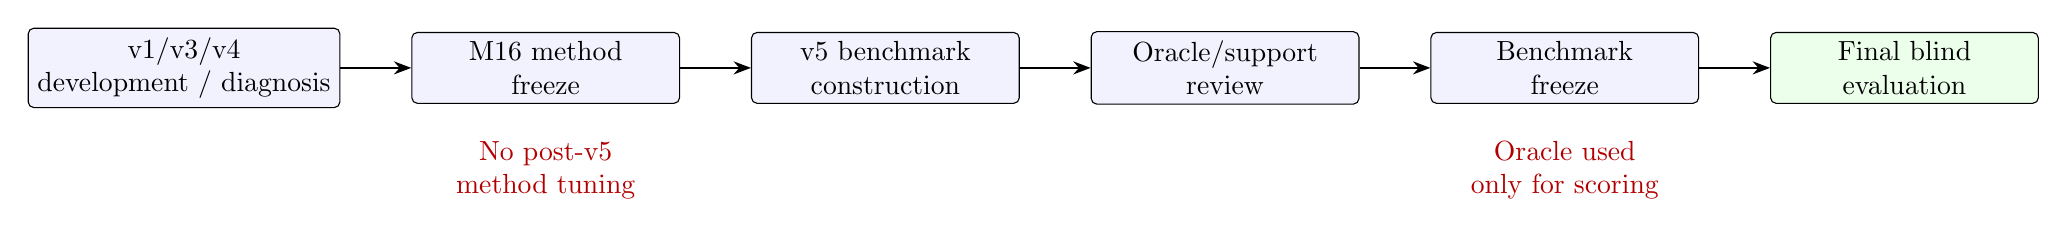
\begin{tikzpicture}[
    node distance=0.9cm,
    stagebox/.style={draw, rounded corners=2pt, align=center, minimum width=3.4cm, minimum height=0.8cm, fill=blue!5},
    eval/.style={draw, rounded corners=2pt, align=center, minimum width=3.4cm, minimum height=0.8cm, fill=green!8},
    arrow/.style={-{Stealth[length=2.2mm]}, thick}
]
\node[stagebox] (dev) {v1/v3/v4\\development / diagnosis};
\node[stagebox, right=of dev] (freeze) {M16 method\\freeze};
\node[stagebox, right=of freeze] (build) {v5 benchmark\\construction};
\node[stagebox, right=of build] (review) {Oracle/support\\review};
\node[stagebox, right=of review] (bfreeze) {Benchmark\\freeze};
\node[eval, right=of bfreeze] (eval) {Final blind\\evaluation};
\draw[arrow] (dev) -- (freeze);
\draw[arrow] (freeze) -- (build);
\draw[arrow] (build) -- (review);
\draw[arrow] (review) -- (bfreeze);
\draw[arrow] (bfreeze) -- (eval);
\node[below=0.35cm of freeze, align=center, red!70!black] {No post-v5\\method tuning};
\node[below=0.35cm of bfreeze, align=center, red!70!black] {Oracle used\\only for scoring};
\end{tikzpicture}}
\caption{方法冻结、benchmark 构建与最终盲测时间线}
\label{fig:timeline}
\end{figure}

\subsection{候选构造协议}

每个事件包含三个候选。Oracle candidate 由公开 evidence 与源 OWL 中待修复断言之间的语义差异生成，表示当前规范证据支持的修复。第一个干扰候选通常保留旧版本、过期值或未修复语义，用于检验系统能否识别语义漂移。第二个干扰候选是语义近邻但不被当前 evidence 最好支持的可执行修复，例如同一 RFC 来源族中的邻近声明、相似作用域或相似规范状态。所有候选都必须满足四个约束：形式化 operation 可执行；OWL patch 可以物化；display value 不包含 oracle、gold、correct 等显式答案标记；candidate note 不被冻结方法读取且经泄漏审计清洗。该协议的目的不是隐藏候选集合，而是保证候选都是形式上可行的竞争修复，从而使评价集中在证据约束的语义选择与 OWL 闭环验证上。

\section{实验设置}

\subsection{比较方法}

本文采用阶段式消融：

\begin{itemize}
    \item \textbf{M13 Base}：包含谓词感知证据聚焦、规则 refinement、Semantic IR 和 V4.3 修复决策。
    \item \textbf{M13+M14}：加入 GRE/CSS recovery。
    \item \textbf{M13+M14+M15}：加入 temporal anchor recovery。
    \item \textbf{ECR-Repair (Full M16 configuration)}：加入 candidate entailment verifier。
\end{itemize}

\subsection{评价指标与统计方法}

主要指标包括 closure accuracy、oracle accuracy 和 strict event accuracy。比例指标使用 Wilson 95\% 置信区间。由于同一事件的 5 次运行共享事件级语义结构，本文同时报告 attempt-level 结果和以事件为独立单位的 event-clustered paired bootstrap。阶段对比的差值置信区间以事件聚类 bootstrap 为主；matched event-run McNemar test 作为配对调用级显著性补充报告。

\subsection{实现细节}

v5 主实验的完整 ECR-Repair 配置见表~\ref{tab:implementation}。M13、M14 和 M16 均使用 DeepSeek API 后端，环境变量 \texttt{DEEPSEEK\_MODEL} 固定为 \texttt{deepseek-chat}，temperature 固定为 0，timeout 为 180 秒。DeepSeek API 不支持严格 seed 控制，因此 seed 只作为审计字段记录。M15 不调用 LLM，是基于公开证据、文档时间元数据和候选盲 IR 的确定性 temporal anchor recovery。OWL/RDF 闭环使用项目中的 RDF graph materialization、reasoner consistency check、graph delta check 和 competency-question regression；任何环节失败都会触发 ABSTAIN。

\begin{table}[t]
\centering
\caption{ECR-Repair v5 主实验实现配置}
\label{tab:implementation}
\resizebox{\linewidth}{!}{%
\begin{tabular}{llll}
\toprule
阶段 & 后端或执行方式 & 主要参数 & 候选可见性 \\
\midrule
M13 Semantic IR Base & DeepSeek API \texttt{deepseek-chat} & temp=0, max tokens=900, timeout=180s & 不可见 \\
M14 GRE/CSS recovery & DeepSeek API \texttt{deepseek-chat} & two JSON calls, 700 tokens each, timeout=180s & 不可见 \\
M15 Temporal anchor recovery & Deterministic recovery & min score=0.30, min margin=0.00, temporal unique top-1 & 不可见 \\
V4.3 Ranking/Gate & Constraint-aware scorer & min score=0.30; GRE/CSS min score=0.24; min margin=0.00; robust IR on & 可见 \\
M16 Candidate verifier & DeepSeek API \texttt{deepseek-chat} & per-candidate call, temp=0, max tokens=500, timeout=180s & 可见 \\
OWL closure & RDF/OWL materialization + reasoner + CQ & candidate OWL, graph delta, consistency, CQ regression & 可见已选候选 \\
\bottomrule
\end{tabular}
}
\end{table}

\section{实验结果}

\subsection{主实验结果}

\begin{table}[t]
\centering
\caption{ECR-Repair 在最终 blind-large benchmark 上的结果}
\label{tab:main}
\begin{tabular}{lccc}
\toprule
语义类型 & Closure & Oracle & Strict event \\
\midrule
ALL & 1319/1320 (99.92\%) & 1319/1320 (99.92\%) & 263/264 (99.62\%) \\
TEMPORAL\_VERSION & 440/440 (100.00\%) & 440/440 (100.00\%) & 88/88 (100.00\%) \\
GENERAL\_RULE\_EXCEPTION & 439/440 (99.77\%) & 439/440 (99.77\%) & 87/88 (98.86\%) \\
CROSS\_SENTENCE\_SCOPE & 440/440 (100.00\%) & 440/440 (100.00\%) & 88/88 (100.00\%) \\
\bottomrule
\end{tabular}
\end{table}

结果显示，ECR-Repair 在最终 blind-large benchmark 上达到 99.92\% closure accuracy 和 99.62\% strict event success。TEMPORAL 和 CSS 两类全部闭环成功，GRE 只剩 1 次调用失败。该结果是在 M16 方法冻结和 v5 benchmark freeze 后取得，因此可作为本文主盲测结果。

\subsection{消融实验}

\begin{table}[t]
\centering
\caption{阶段式消融实验}
\label{tab:ablation}
\begin{tabular}{lcccc}
\toprule
方法阶段 & Closure & Strict event & 相对 M13 提升 & 阶段增益 \\
\midrule
M13 Base & 1022/1320 (77.42\%) & 195/264 (73.86\%) & 0.00 pp & -- \\
M13+M14 & 1058/1320 (80.15\%) & 205/264 (77.65\%) & 2.73 pp & 2.73 pp \\
M13+M14+M15 & 1305/1320 (98.86\%) & 261/264 (98.86\%) & 21.44 pp & 18.71 pp \\
ECR-Repair & 1319/1320 (99.92\%) & 263/264 (99.62\%) & 22.50 pp & 1.06 pp \\
\bottomrule
\end{tabular}
\end{table}

消融结果说明每个模块均有明确贡献。M14 主要提升 GRE/CSS 的失败子集；M15 针对早期开发阶段识别出的 temporal anchor ambiguity 进行恢复，并在冻结后的 v5 blind-large benchmark 上表现出最大的阶段增益；M16 进一步修复最后的 GRE candidate entailment 边界案例。

\subsection{候选选择 Baseline}

为检验最终结果是否仅来自候选集合本身过于明显，本文补充两个全量候选选择 baseline。二者均读取公开 evidence、事件元数据和候选集合，但不执行本文的 Semantic IR 分层修复、选择性门控、OWL patch、reasoner 和 CQ closure。\texttt{OPTION\_VALUE\_ONLY} 只向模型提供候选 display value；\texttt{OPTION\_FORMAL\_OPERATION} 提供候选 display value 和形式化 operation object。

\begin{table}[t]
\centering
\caption{全量候选选择 baseline 与 ECR-Repair 对比}
\label{tab:baselines}
\begin{tabular}{lccc}
\toprule
方法 & Oracle selection & OWL closure & 备注 \\
\midrule
OPTION\_VALUE\_ONLY & 1234/1320 (93.48\%) & -- & evidence + candidate value \\
OPTION\_FORMAL\_OPERATION & 1171/1320 (88.71\%) & -- & evidence + formal operation \\
M13 Base & 1022/1320 (77.42\%) & 1022/1320 (77.42\%) & 基础 Semantic IR 修复管道 \\
ECR-Repair & 1319/1320 (99.92\%) & 1319/1320 (99.92\%) & 完整 OWL 闭环修复 \\
\bottomrule
\end{tabular}
\end{table}

结果表明，v5 benchmark 并非只靠候选值即可自然达到接近满分。ECR-Repair 比最强简单 baseline \texttt{OPTION\_VALUE\_ONLY} 高 6.44 个百分点。若按错误率计算，\texttt{OPTION\_VALUE\_ONLY} 的错误率为 6.52\%，ECR-Repair 的错误率为 0.08\%，相当于将残余错误压缩约 98.84\%。对 M13 和 ECR-Repair 而言，Oracle selection 与 OWL closure 相同，说明被正确选择的候选均通过了形式化闭环。

\subsection{统计显著性与置信区间}

\begin{table}[t]
\centering
\caption{ECR-Repair Wilson 95\% 置信区间}
\label{tab:ci}
\begin{tabular}{llcc}
\toprule
语义类型 & 指标 & 估计值 & Wilson 95\% CI \\
\midrule
ALL & Attempt closure & 99.92\% & 99.57--99.99\% \\
ALL & Strict event closure & 99.62\% & 97.89--99.93\% \\
TEMPORAL\_VERSION & Attempt closure & 100.00\% & 99.13--100.00\% \\
TEMPORAL\_VERSION & Strict event closure & 100.00\% & 95.82--100.00\% \\
GENERAL\_RULE\_EXCEPTION & Attempt closure & 99.77\% & 98.72--99.96\% \\
GENERAL\_RULE\_EXCEPTION & Strict event closure & 98.86\% & 93.84--99.80\% \\
CROSS\_SENTENCE\_SCOPE & Attempt closure & 100.00\% & 99.13--100.00\% \\
CROSS\_SENTENCE\_SCOPE & Strict event closure & 100.00\% & 95.82--100.00\% \\
\bottomrule
\end{tabular}
\end{table}

\begin{table}[t]
\centering
\caption{阶段增益的事件聚类配对统计检验}
\label{tab:tests}
\begin{tabular}{lccc}
\toprule
对比 & 平均提升 & Event-clustered 95\% CI & Attempt-level paired McNemar $p$ \\
\midrule
ECR-Repair vs M13 & 22.50 pp & 17.73--27.42 pp & $7.85\times10^{-90}$ \\
M13+M14 vs M13 & 2.73 pp & 1.06--4.70 pp & $2.91\times10^{-11}$ \\
M13+M14+M15 vs M13+M14 & 18.71 pp & 14.32--23.41 pp & $8.84\times10^{-75}$ \\
ECR-Repair vs M13+M14+M15 & 1.06 pp & 0.00--2.42 pp & $1.22\times10^{-4}$ \\
\bottomrule
\end{tabular}
\end{table}

ECR-Repair 相比 M13 Base 的提升达到 22.50 个百分点，在事件聚类 bootstrap 下 95\% 置信区间为 17.73--27.42 个百分点。M16 相对 M13+M14+M15 的最后增益较小，其事件聚类置信区间下界为 0.00 pp，因此应解释为减少残余失败的保守验证层，而不是主要增益来源。

\subsection{选择性修复指标}

\begin{table}[t]
\centering
\caption{Coverage、abstention 与 selected precision}
\label{tab:selective}
\begin{tabular}{lcccc}
\toprule
方法 & Coverage & Abstention & P(Oracle $\mid$ Select) & Wrong selected \\
\midrule
M13 Base & 1034/1320 (78.33\%) & 286/1320 (21.67\%) & 1022/1034 (98.84\%) & 12/1320 (0.91\%) \\
ECR-Repair & 1319/1320 (99.92\%) & 1/1320 (0.08\%) & 1319/1319 (100.00\%) & 0/1320 (0.00\%) \\
\bottomrule
\end{tabular}
\end{table}

选择性修复结果显示，ECR-Repair 不只是提高覆盖率，还保持了选中条件下 100.00\% 的 oracle precision。唯一失败为 abstain，因此没有不受证据支持的错误 OWL patch。

\subsection{鲁棒性实验}

为检验候选顺序和候选编号是否驱动结果，本文在 v5 benchmark 上构建两个派生扰动副本：candidate-order-shuffle 只打乱每个事件的候选行顺序，candidate-id-rename 将候选编号一致替换为中性 \texttt{ALT\_A}/\texttt{ALT\_B}/\texttt{ALT\_C} 并同步重写 private Oracle。原始 benchmark 不被修改。在线鲁棒性实验覆盖全部 264 个事件、每个事件 5 次运行，即每个扰动 1320 次调用，并运行完整 M13--M16 管道。

\begin{table}[t]
\centering
\caption{v5 全量在线候选扰动鲁棒性实验}
\label{tab:online-robustness}
\begin{tabular}{lcc}
\toprule
实验条件 & Closure & Strict event \\
\midrule
原始 v5 & 1319/1320 (99.92\%) & 263/264 (99.62\%) \\
candidate-order-shuffle & 1317/1320 (99.77\%) & 261/264 (98.86\%) \\
candidate-id-rename & 1313/1320 (99.47\%) & 261/264 (98.86\%) \\
\bottomrule
\end{tabular}
\end{table}

结果显示，候选顺序扰动下 closure 仍为 99.77\%，候选编号重命名下 closure 为 99.47\%。因此，方法并非简单依赖候选文件原始顺序或固定 \texttt{CAND\_002} 编号；但扰动结果并非完全不变，剩余失败集中在 GRE/CSS 的 fail-closed 或 abstain 边界案例。作为补充，本文还对 v5 主结果中 M13/V4.3 score-based ranking 层进行离线 replay，具有 candidate score 记录的 1101 行中，candidate id rename 后 top candidate 映射保持不变；另有 219 行不适用。candidate notes 泄漏审计显示，清洗后 792 行候选 notes 中泄漏行数为 0，且冻结方法文件没有读取 candidate notes。

\subsection{泛化实验}

Domain 级别上，11 个领域中有 10 个达到 100\% closure，唯一非满分领域为 \texttt{dns\_security}，达到 119/120，即 99.17\%。Source-family 级别上，13 个实际入选 RFC 来源族中有 12 个达到 100\%，唯一非满分来源族为 \texttt{IETF RFC 4035}，达到 119/120，即 99.17\%。

\begin{table}[t]
\centering
\caption{冻结方法的领域分组结果}
\label{tab:domain}
\begin{tabular}{lccc}
\toprule
Domain & Events & Closure & Strict event \\
\midrule
dns\_security & 24 & 119/120 (99.17\%) & 23/24 (95.83\%) \\
email\_authentication & 24 & 120/120 (100.00\%) & 24/24 (100.00\%) \\
http\_messaging & 24 & 120/120 (100.00\%) & 24/24 (100.00\%) \\
http\_semantics & 24 & 120/120 (100.00\%) & 24/24 (100.00\%) \\
internationalized\_identifiers & 24 & 120/120 (100.00\%) & 24/24 (100.00\%) \\
json\_formats & 24 & 120/120 (100.00\%) & 24/24 (100.00\%) \\
oauth\_authorization & 24 & 120/120 (100.00\%) & 24/24 (100.00\%) \\
privacy\_considerations & 24 & 120/120 (100.00\%) & 24/24 (100.00\%) \\
security\_considerations & 24 & 120/120 (100.00\%) & 24/24 (100.00\%) \\
tls\_security & 24 & 120/120 (100.00\%) & 24/24 (100.00\%) \\
uri\_templates & 24 & 120/120 (100.00\%) & 24/24 (100.00\%) \\
\bottomrule
\end{tabular}
\end{table}

需要强调的是，该实验应表述为 frozen-method domain/source-family test-slice evaluation，而不是训练式 leave-one-domain-out learning experiment。因为本文方法没有针对每个 domain 重新训练模型。

\subsection{模型后端对比}

作为补充后端鲁棒性实验，本文在 \texttt{external-real-holdout-v3-large} 上比较了 DeepSeek 云端模型和 Ollama 本地 \texttt{qwen3.5:9b}。该实验与上文 264 事件的 \texttt{external-real-holdout-v5-blind-large} 主结果属于不同实验版本，不能混作同一主结果。结果显示：

\begin{itemize}
    \item Ollama closure：1085/1100，98.64\%；
    \item DeepSeek closure：1091/1100，99.18\%；
    \item 两者 strict event 均为 217/220。
\end{itemize}

这说明方法并非完全依赖某个云端大模型。两个后端在 attempt 级别存在少量差异，但 strict event 级别表现相同。

\subsection{失败案例分析}

最终 v5 blind-large 实验中只剩 1 次失败，来自事件 \texttt{H5\_E017} 的第 5 次运行。该事件属于 \texttt{GENERAL\_RULE\_EXCEPTION}，失败表现为 M16 candidate entailment verifier 未找到唯一被证据支持的候选，因此选择 abstain。

\begin{table}[t]
\centering
\caption{最终主实验与全量扰动实验的剩余失败}
\label{tab:failures}
\begin{tabular}{llcc}
\toprule
实验 & 主要事件 & 失败调用 & 解释 \\
\midrule
原始 ECR-Repair & H5\_E017 & 1 & GRE tie-abstain \\
candidate-order-shuffle & H5\_E003/H5\_E207/H5\_E257 & 3 & GRE/CSS fail-closed 或 abstain \\
candidate-id-rename & H5\_E003/H5\_E017/H5\_E137 & 7 & GRE/CSS fail-closed 或 abstain \\
\bottomrule
\end{tabular}
\end{table}

因此，最终错误不是 JSON 格式问题，也不是 TEMPORAL 的系统性失败，而是 GRE/CSS 边界样本中的证据蕴含或候选区分不确定性。所有剩余失败均以 abstain 或 fail-closed 结束，没有产生错误 OWL patch。

\begin{table}[t]
\centering
\caption{M13 Base 与 ECR-Repair 的失败链路分布}
\label{tab:failure-flow}
\begin{tabular}{lcc}
\toprule
失败或成功状态 & M13 Base & ECR-Repair \\
\midrule
IR invalid 或 incomplete & 219 & 0 \\
Rank/tie abstain & 67 & 1 \\
Wrong select & 12 & 0 \\
OWL closure fail after correct select & 0 & 0 \\
Success & 1022 & 1319 \\
\bottomrule
\end{tabular}
\end{table}

失败链路分布说明，ECR-Repair 主要压缩的是 M13 中的 IR 不完整、排序弃权和平局弃权，同时没有引入错误选择或形式化闭环失败。

\begin{figure}[t]
\centering
\resizebox{0.88\linewidth}{!}{%
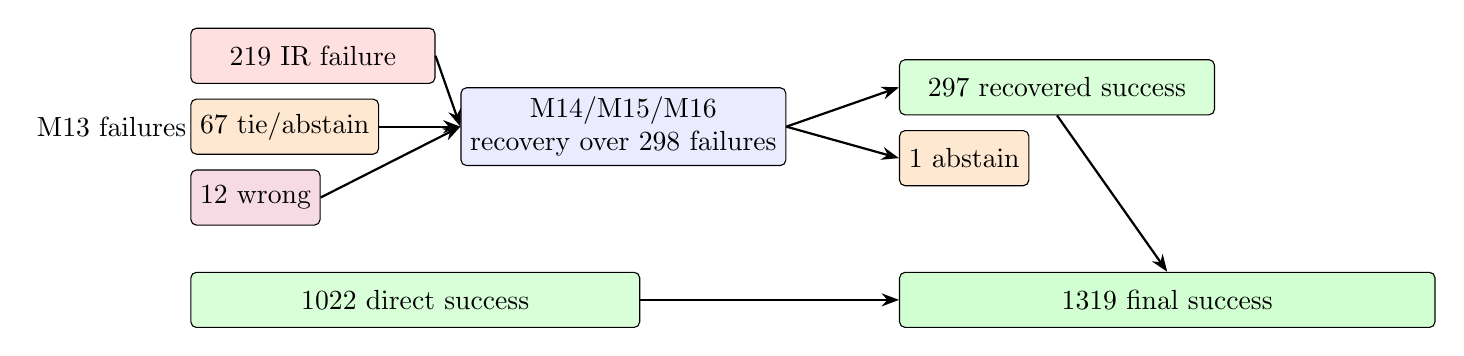
\begin{tikzpicture}[
    bar/.style={draw, rounded corners=2pt, minimum height=0.7cm, align=left},
    label/.style={align=right},
    arrow/.style={-{Stealth[length=2.2mm]}, thick}
]
\node[label] at (0,0.2) {M13 failures};
\node[bar, fill=red!12, minimum width=3.1cm, anchor=west] (m13ir) at (1,1.1) {219 IR failure};
\node[bar, fill=orange!18, minimum width=1.5cm, anchor=west] (m13tie) at (1,0.2) {67 tie/abstain};
\node[bar, fill=purple!14, minimum width=0.9cm, anchor=west] (m13wrong) at (1,-0.7) {12 wrong};
\node[bar, fill=green!15, minimum width=5.7cm, anchor=west] (m13ok) at (1,-2.0) {1022 direct success};
\node[bar, fill=blue!8, minimum width=3.8cm, align=center] (recovery) at (6.5,0.2) {M14/M15/M16\\recovery over 298 failures};
\node[bar, fill=green!15, minimum width=4.0cm, anchor=west] (recok) at (10.0,0.7) {297 recovered success};
\node[bar, fill=orange!18, minimum width=0.7cm, anchor=west] (recfail) at (10.0,-0.2) {1 abstain};
\node[bar, fill=green!18, minimum width=6.8cm, anchor=west] (m16ok) at (10.0,-2.0) {1319 final success};
\draw[arrow] (m13ir.east) -- (recovery.west);
\draw[arrow] (m13tie.east) -- (recovery.west);
\draw[arrow] (m13wrong.east) -- (recovery.west);
\draw[arrow] (recovery.east) -- (recok.west);
\draw[arrow] (recovery.east) -- (recfail.west);
\draw[arrow] (m13ok.east) -- (m16ok.west);
\draw[arrow] (recok.south) -- (m16ok.north);
\end{tikzpicture}}
\caption{失败模式从 M13 Base 到 ECR-Repair 的逐层压缩}
\label{fig:failure-flow}
\end{figure}

\section{讨论}

实验表明，本任务的关键不是简单保证 LLM 输出 JSON 格式正确。早期实验已经发现，强制结构化输出虽然可以提高 parse rate，但可能导致语义失真。本文最终方法通过拆分 evidence focus、task formulation、Semantic IR、candidate-blind normalization、candidate-aware ranking 和 formal closure，使得每个失败都可以定位到具体模块。

从消融结果看，M14、M15 和 M16 分别解决不同类型的瓶颈。M14 对 GRE/CSS 边界问题有效，M15 针对早期开发阶段识别出的 temporal anchor ambiguity，并在 v5 上显示出最大泛化增益；M16 进一步通过 entailment verifier 修复最后一批候选语义判别问题。attempt-level McNemar test 显示 M16 相对 M13+M14+M15 的差异显著，而 event-clustered bootstrap 的下界达到 0，说明该增益在事件级推断下应保守解释为残余失败压缩。最终剩余失败为单次 GRE abstain，说明在当前 frozen RFC benchmark 上，主要系统性失败模式已被显著压缩。

考虑到最终 closure accuracy 接近满分，本文进一步检查 benchmark 难度和候选泄漏等替代解释。首先，主结果不是在方法开发用的 v1/v3/v4 数据集上取得，而是在 M16 方法冻结后重新构建、复核并 freeze 的 v5 blind-large 数据集上取得。其次，candidate notes 在公开发布前被统一清洗，冻结方法不读取 notes 字段；Oracle 位于 private 路径，只在预测固定后用于计分。再次，M13 Base 只有 77.42\% closure，说明仅依靠公开证据和基础 Semantic IR 并不能自然达到接近满分；M14--M16 的逐步提升来自明确的新增机制，而不是简单任务本身。最后，唯一剩余错误以 abstain 结束，说明 safety gate 仍保持 fail-closed，而不是为了追求准确率强行选择候选。

\section{有效性威胁}

\textbf{来源领域限制。} 最终 benchmark 主要来自 RFC/IETF 风格的公开技术规范。虽然覆盖 11 个 domain 和 13 个实际入选 RFC 来源族，但不能直接推出对所有法律、监管或行业规范文本都有效。本文结论应限定为版本化技术规范文档中的证据约束 OWL 修复；迁移到法规、合同、临床指南等更强语境依赖的文本时，需要重新构建 domain vocabulary、candidate generation protocol 和独立 hold-out。

\textbf{数据构造限制。} v5 benchmark 使用真实公开 RFC 文档和原始 evidence window，但 repair event、subject/predicate metadata 与候选集合仍由实验协议构造。因此本文验证的是已知潜在漂移事件条件下的证据约束修复，而不是从完整文档库中自动发现全部漂移事件。若要主张完整 semantic drift detection，还需要另行补充 discovery-level precision、recall 和 F1 实验。

\textbf{schema 依赖。} 方法使用 semantic type、任务表述路由和领域级规范词汇，因此不能声称是完全自动的开放域规则学习系统。

\textbf{oracle 复核限制。} 当前 benchmark 使用单人复核。虽然已有 evidence window、freeze manifest 和 private oracle isolation，但未来仍应增加多标注者一致性分析。

\textbf{领域分组表述边界。} 当前 domain/source-family 实验是冻结方法后的测试切片分析，不是每个 domain 重新训练后的 transfer learning 实验。

\textbf{candidate notes 泄漏处理。} 早期候选 notes 含有 oracle 暗示文本。该问题已通过 post-sanitize 清洗修复，审计显示泄漏行为 0，且离线 scoring 证明清洗不改变最终结果。论文和公开材料必须只使用清洗后的 benchmark manifest。

\textbf{最终盲测边界。} 本文将早期 v1/v3/v4 数据集定位为诊断、校准或验证数据。最终主结果使用 M16 冻结后重新构建并 freeze 的 v5 blind-large benchmark。后续若继续修改方法，必须再构建新的独立数据集，不能继续把 v5 作为最终盲测。

\section{结论}

本文提出一种面向版本化规范文档的证据约束语义中间表示本体修复方法。该方法将 LLM 的规范文本理解能力与候选隔离、约束感知排序、选择性安全门控和 OWL 形式化验证结合起来。在 264 个基于真实 RFC 规范文档构建并人工复核的修复事件、1320 次调用的最终 blind-large 实验中，ECR-Repair 达到 99.92\% closure accuracy 和 99.62\% strict event success。消融、统计检验、鲁棒性、领域分组和失败分析共同表明，该方法能够稳定地将版本化规范证据转化为可审计的 OWL 修复决策。

\bibliographystyle{plain}
\bibliography{references}

\end{document}


